\documentclass[11pt]{scrartcl}

\usepackage[T1]{fontenc}
\usepackage[utf8]{inputenc}
\usepackage{lmodern}
\usepackage[english]{babel}
\usepackage{xcolor}
\usepackage{amsmath}
\usepackage{amssymb}
\usepackage{amsfonts}
\usepackage{amsthm}
\usepackage[centerdot]{mathtools}
\usepackage{hyperref}
\usepackage{tikz}
\usepackage[ruled]{algorithm2e}
\SetKw{Continue}{continue}
\SetKw{Null}{null}
\SetKw{Break}{break}
\usepackage[textsize=tiny]{todonotes}
\usepackage[normalem]{ulem}
\usepackage{float}
\usepackage{subfig}
\usepackage{pgfplots}
\usepackage{booktabs,caption}
\usepackage[flushleft]{threeparttable}

\newcommand{\daniel}[1]{\todo[linecolor=blue,backgroundcolor=blue!25]{#1}}
\newcommand{\david}[1]{\todo[linecolor=orange,backgroundcolor=orange!25]{#1}}
\newcommand{\laura}[1]{\todo[linecolor=green,backgroundcolor=green!25]{#1}}
\newcommand{\moritz}[1]{\todo[linecolor=red,backgroundcolor=red!25]{#1}}
\newcommand{\changedByLP}[1]{\textcolor{green!50!black}{#1}}
\newcommand{\changedByDP}[1]{\textcolor{blue!50!black}{#1}}
\newcommand{\changedByDK}[1]{\textcolor{orange!50!black}{#1}}
\newcommand{\changedByMW}[1]{\textcolor{red!50!black}{#1}}

\DeclareMathOperator{\cost}{cost}

%\numberwithin{equation}{section}
\newtheorem{theorem}{Theorem}[section]
\newtheorem{lemma}[theorem]{Lemma}
\newtheorem{definition}[theorem]{Definition}
\newtheorem{property}[theorem]{Property}

\title{Pool Trading for Hybrid Wind-Solar Power Producers}
%alternative: The all optimal integer flow problem and its applications.
\author{David K\"onen, Daniel Piersig, Laura Poreschack, Moritz Wegener  }  % in alphabetical order
%\keywords{All integer optimal flow problem; networkflow; minimum cost flow problem}


\begin{document}

\maketitle

\begin{abstract}
		This survey addresses a pool trading decision problem for a hybrid power producer producing both wind power and solar power collectively. To solve the decision problem the hybrid producer has to face, we will solve a scenario-based two-stage optimisation problem based on the model out of \cite{Conejo10}. We will consider two situations: one adding an adjustment market and one without an adjustment market. Also, we will compare our optimisation results for the hybrid power producer with the results only considering one energy resource separately.  For generating wind and solar power scenarios, we use a time-series-based approach on a historical data set from Germany \cite{url}. We will exploit an anti-correlation of wind and solar power generation. Due to this anti-correlation, we will see that the hybrid power producer faces fewer variances in power production and hence can offer more power  to a given day-ahead price with less risk. Moreover, we will show that the more risk-averse a producer is, the more profitable it is to produce in a hybrid scheme. 
\end{abstract}

 %Section1 Introduction
 \section{Introduction}

Renewable energies are currently advancing and gaining an increasing share of the energy production. On the one hand, this is induced by the desire to decrease the carbon footprint and on the other hand, the population is facing a decreasing availability of fossil fuels like natural gas, coal and oil. The advantage of renewable energies is that apart from not requiring fuel, which induces zero fuel costs, it is emission-free and therefore supported by the government. However, these energy sources are also non-dispatchable and have the major disadvantage of uncertainty. Conejo et al. \cite{Conejo10} considered the case of a wind power producer. Due to the uncertainty, the wind power producer must rely on the energy traded on the balancing market. Therefore, he solved an optimisation problem to maximise the expected profits from trading on the day-ahead market and the adjustment market while also minimising the costs incurred in the balancing market caused by energy deviations. 

In addition to the uncertainty, the wind power producer also faces a substantial fluctuation in production throughout the year, caused by the strong dependence on wind availability over different months in a year. Considering a wind power producer in Europe, wind availability is much higher in the winter than summer months, see, e.g. \cite{W11}. 

For this case study, we consider the case of an energy producer producing both wind power as well as solar energy. Several studies have been carried out to see how both resources' production variability  can be decreased by exploiting the anti-correlation of wind speed and solar irradiance. Coker et al. \cite{Coker2013} considered a region in south-west Britain to assess the variability of wind, solar and tidal current energy resources. Santos-Alamillos et al. \cite{Santos-Alamillos} aimed at finding the optimal spatial distribution of wind and solar farms across the Southern Iberian Peninsula to minimise the resulting net variability. Bett et al. \cite{BETT16} analysed daily data for Great Britain and found  evidence for an overall anticorrelation between wind speed and solar irradiance. As a side product, they also discovered that solar variability is significantly higher than wind variability and that both variabilities are higher in winter than in summer. Inspired by these results, we wish to set up a pool trading model for an energy producer offering energy produced from both solar and wind power plants.  
This setting of a hybrid wind-solar power producer
	overcomes the strong fluctuation in production throughout the year due to the strong over year anti-correlation of wind speed and solar irradiance, see figure \ref{fig:overyear}. In addition to
	the anti-correlation between wind speed and solar irradiance over the whole year, there is also an anti-correlation between both over the day, even if it is much smaller. We will exploit this anti-correlation over the day and include it into the forecast
	for wind and solar power production. Therefore, we will apply the forecast for wind power production for a time $t$ in dependence on the previous times' wind speeds and previous times' solar irradiance to improve the forecast precision possibly.

	
\begin{figure}[h!]
	\centering
	
	\begin{minipage}{0.8\textwidth}
		\subfloat{
			\centering
			\scalebox{0.4}{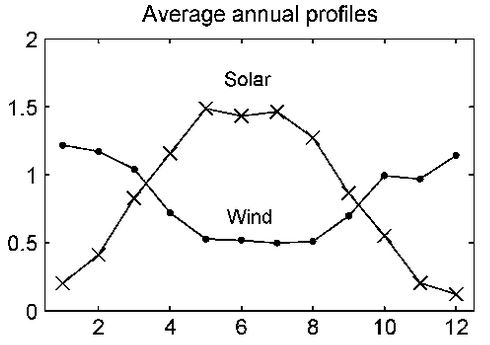
\includegraphics{Figures/year.jpg}}
		}
		\hfill
		\subfloat{
			\centering
			\scalebox{0.4}{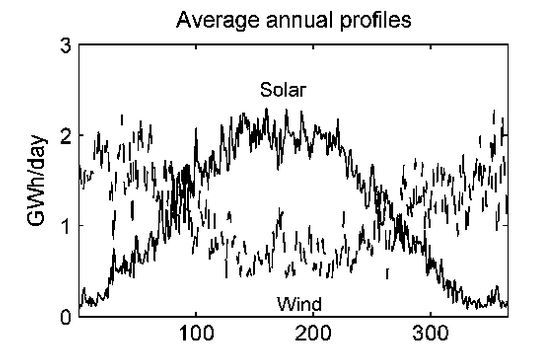
\includegraphics{Figures/year2.png}}
		}
		
		\caption{The average annual profiles of solar irradiance and wind speed \cite{W11}}\label{fig:overyear}
	\end{minipage}	
\end{figure}
To solve the  decision problem, the hybrid energy producer has to face, we will solve a scenario-based multi-stage optimization problem. For generating wind and solar power scenarios, we will use a time-series-based approach on a historical data set. With the generated data, we consider two cases. First, we look at a situation where we do not have an adjustment market. Second, we add an adjustment market to our situation. We compare the revenue of a hybrid producer with the sum of the revenues of a solar and a wind power producer. Our results show that the more risk averse a producer is, the more profitable it is to produce in a hybrid scheme. This effect can be observed in both market situations. We conclude that this profitability stems from the anit-correlation of the two weather conditions as a decrease in availability of solar irradiance is most likely to be compensated by an increase of wind speed and vice versa. This gives more planning security and therefore a higher expected profit. Moreover, the decrease in planning insecurity also explains why more risk averse producers profit more from a hybrid production scheme.  

 
 
 %Section 2 Decision Framework
 \section{Decision framework}
In the introduction we mentioned the three major trading places for energy, namely the day-ahead, the adjustment and the balancing market. All three of these are cleared in a single auction process, however at different times of the day. 

\begin{list}{$\cdot$}{}
	\item The day-ahead market is cleared at a given time period $t^D$ of day $d-1$.
	\item The adjustment market is cleared at time period $t^{A}$ of day $d-1$. Please note that time period $t^{A}$ takes place \textit{after} time period $t^{D}$.
	\item The balancing market ensures the real-time balancing between the generation of and demand for energy by balancing out differences between the real-time operation and the last energy program settled on in the previous markets. Therefore, it is cleared just before each time period of day $d$. 
\end{list}
There are three major decision the hybrid energy producer has to face. First, he has to submit an offering curve to the day-ahead market for each time period of day $d$. Then, he has to modify the submitted energy offers in the adjustment market depending on how the wind and solar power forecast updates change. Finally, he balances out his energy deviations by trading in the balancing market for each time period of day $d$. From now on, we assume hourly periods. This means that the balancing market for the time period 6.00-7.00 am of day $d$ closes at 5.50 am of day $d$. 
\\
\\ The producer faces several factors that influence his short-term decision making process. It is inevitable to account for the imbalance costs, i.e. the costs entailed bx deviations in the energy production. Apart from that, he is influenced by all sorts of mechanisms through which energy deviations are priced in the balancing market and the beneficial impact of an adjustment market clearing after the clearance of the day-ahead market. Energy deviations are not unusual for producers of non-dispatchable energy sources as windspeed and solar irradiance exert a high variability. As soon as a producer deviates from his agreed-upon amount of energy he had traded on the market before, he has to sell its surplus or buy his generation deficit at an \textit{imbalance price}. We denote the price for positive energy deviations, i.e. higher production than planned, by $\lambda_{t}^{+}$ and the price for negative energy deviations by $\lambda_{t}^{-}$. If the producer faces a negative system imbalance $\delta_{t}$, which means there is a deficit of energy generation, we have
\begin{align*}
	&\lambda_{t}^{+}=\lambda_{t}^{D}
	\\ &\lambda_{t}^{-}=max\left(\lambda_{t}^{D}, \lambda_{t}^{UP}\right),
\end{align*}
where we write $\lambda_{t}^{D}$ for the day-ahead market price and $\lambda_{t}^{UP}$ for the price of the upward energy that needs to be added to the system. In case of a generation excess in the power system, i.e. $\delta_{t}>0$, we have 
\begin{align*}
	&\lambda_{t}^{+}=min\left(\lambda_{t}^{D}, \lambda_{t}^{DOWN}\right)
	\\ &\lambda_{t}^{-}=\lambda_{t}^{D}.
\end{align*} 
Here, $\lambda_{t}^{DOWN}$ is the parameter for the price of the downward energy that has to be removed from the system. 
\\ \\
The producer offers an amount $E_{t}^{D}$ of energy at the day-ahead market, while his plant produces an emount $E_{t}$, which is most probably not equal to the amount offered at the day-ahead market. Hence, he expects a revenue of
\begin{equation*}
	R_{t}=\lambda_{t}^{D}\cdot E_{t}^{D} + I_{t},
\end{equation*}
where we write $I_{t}$ for the imbalance income. Note that this can be either positive or negative depending on the market imbalance and the production imbalance. We denote the total deviation by
\begin{equation*}
	\Delta_{t}=E_{t}-E_{t}^{D}=d_{t}\left(P_{t}-P_{t}^{D}\right)
\end{equation*}
indicating the timespan by $d_{t}$ and the actual resp. offered amount of power by $P_{t}$ resp. $P_{t}^{D}$. Applying this notation, we can write
\begin{align*}
	I_{t}= \begin{cases}
		\lambda_{t}^{+}\Delta_{t} &\mathrm{\; if \;} \Delta_{t} \geq 0,
		\\ \lambda_{t}^{-}\Delta_{t} &\mathrm{\; if \;} \Delta_{t}\leq 0
	\end{cases}
\end{align*}
and define the ratios 
\begin{equation*}
	r_{t}^{+}= \frac{\lambda_{t}^{+}}{\lambda_{t}^{D}} \mathrm{\; and \;} r_{t}^{-}=\frac{\lambda_{t}^{-}}{\lambda_{t}^{D}}.
\end{equation*}
Thus, the revenue can be rewritten as
\begin{align*}
	R_{t}= \begin{cases}
		\lambda_{t}^{+}\left(E_{t}\right)+\lambda_{t}^{D}r_{t}^	{+}\Delta_{t} &\mathrm{\; if \;} \Delta_{t} > 0,-\Delta_{t}
		\\ \lambda_{t}^{+}\left(E_{t}\right)+\lambda_{t}^{D}r_{t}^	{-}\Delta_{t} &\mathrm{\; if \;} \Delta_{t}< 0
	\end{cases}
\end{align*} 
In general, we can also formulate the revenue in terms of the maximum level of revenue, which could be realised in a situation free of wind and irradiance uncertainty, and the imbalance cost, which we define as $C_{t}$
\begin{equation*}
	C_{t}=\begin{cases}
		\lambda_{t}\left(1-r_{t}^{+}\right)\Delta_{t} &\mathrm{\; if \;} \Delta_{t}>0
		\\ -\lambda_{t}^{D}\left(r_{t}^{--1}\right)\Delta_{t} &\mathrm{\; if \;} \Delta_{t}<0.
	\end{cases}
\end{equation*}
This characterisation renders it possible to give a more concise formulation of the revenue 
\begin{equation*}
	R_{t}=\lambda_{t}^{D}E_{t}-C_{t},
\end{equation*}
which makes it easy to deduce that maximising the revenue is equivalent to minimising the imbalance costs. 
\\ \\
We face four major sources of uncertainty. The most essential source of uncertainty is the weather, which influences both the wind and solar power generation. Apart from that, we have uncertainty concerning the market characteristics like day-ahead market price, adjustment market price and the prices for imbalance.
For our purpose, we consider $N_{T}$ periods of the market horizon, $N_{D}$ scenarios for day-ahead prices and $N_{A}$ scenarios for the adjustment market prices. Thus, we have several realisations of day-ahead and adjustment market prices, which we summarise in
\begin{align*}
	\lambda^{D}=\left\{\lambda_{t}^{D} \quad \lvert \quad t \in \left\{1, .., N_{T}\right\}\right\}
	\\ \lambda^{A}=\left\{\lambda_{t}^{A}\quad \lvert \quad t \in \left\{1, .., N_{A}\right\}\right\}.
\end{align*}
The hybrid power producer has to adhere the following sequence of decisions. First, the designs an offer strategy for the day-ahead market and submits his selling offers for each period of the market horizon. Second, once the day-ahead market is known for each time period, he has to decide on the amount of energy that he wishes to sell or buy from the adjustment market. As soon as the adjustment market prices are known as well as the imbalance prices and the generated wind and solar power, the producer knows his level of imbalance and can compute the resulting costs for the latter.  


 %Section 3 Case Study
 
\section{Case Study}

\subsection{Scenario Generation}
As already mentioned in subsection \ref{sub:Uncertainty_Characterization} our model has to account for variations concerning solar and wind power generation in between the clearance of the day-ahead and adjustment market $\overline{P}^{W}$,$\overline{P}^{S}$ and during the market horizon ${P}^{W}$, ${P}^{S}$ as well as the prices at the day-ahead and adjustment market $\lambda^D$, $\lambda^A$ and the imbalance price ratios $r^+$,$r^-$. Market prices are assumed to be independent of power generation. However, interdependencies within the sets of $\left\lbrace\overline{P}^{W},{P}^{W},\overline{P}^{S},{P}^{S}\right\rbrace$ and $\left\lbrace\lambda^D,\lambda^A,r^+,r^-\right\rbrace$ respectively can not be neglected. Without losing generality, we limit our analysis to a single time period 12:00 PM - 13:00 PM. Furthermore, for simplicity, we utilize the market scenario of page 220 \cite{Conejo10}. %but extend it by a second version where $E\left[\lambda^D-\lambda^A\right]<0$
Our goal is to model an even split between solar and wind energy on an average day concerning power generation. To do so, we analyze historical data from the 50Hertz control area in Germany  \cite{url}. The data set supplies hourly power generation from 01. January 2015 to 01. October 2020. As mentioned before, solar and wind power generation is strongly dependent on the weather and exhibits strong seasonal effects. While such seasonal effects have interesting economic implications on their own, they should not drive the variance of power generation in our scenarios. In other words, making use of scenarios that best represent the market for a variety of seasons would exaggerate the spread in power generation and hence not represent the energy market at any day throughout the analyzed period. Furthermore, in the data set, the average power generation from wind is 216\% higher than the solar power generation. To mitigate the skewness towards wind energy and the seasonal effects, we first normalize the average power generation of both supply streams to $5.000 MW$. Second, we subtract the 30-day moving average and reapply the overall average $\left(\sim 5.000 MW\right)$. Note that our model solar energy will nevertheless outweigh wind energy due to our focus on the 12:00 PM - 13:00 PM market horizon. To account for the negative correlation between solar and wind power generation, we fit both supply streams to ARMA models of the form $y_t = \mu + \phi \left(y_{t-1}-\mu\right)+\varepsilon_t + \theta\varepsilon_{t-1}$ and compute the variance-covariance Matrix $G$ of $\varepsilon^S$ and $\varepsilon^W$, where $\varepsilon^S$ $\left(\varepsilon^W\right)$ refers to the residual vector of the solar (wind) energy ARMA model. The stochastic processes 
for solar and wind energy supply can hence be described as follows:

\begin{align}
\overline{P}^{W}=& \mu^W+\epsilon_1^W\\
\overline{P}^{S}=& \mu^S+\epsilon_1^S\\
{P}^{S}=&\mu^S + \phi^S \left(\overline{P}^{S}-\mu^S\right)+\epsilon^S_2 + \theta^S\epsilon^S_1\\
{P}^{W}=&\mu^W + \phi^W \left(\overline{P}^{W}-\mu^W\right)+\epsilon^W_2 + \theta^W\epsilon^W_1.
\end{align}


Note again, that $\varepsilon^S$ and $\varepsilon^W$ refer to the residual vectors from the fitted ARMA models while $\left(\epsilon_1^S,\epsilon_1^W\right)$ and $\left(\epsilon_2^S,\epsilon_2^W\right)$ correspond to two independent realizations of the same random variable distributed according to a multivariate normal distribution with variance-covariance matrix $G$ and mean $\overline{\varepsilon}^S$, $\overline{\varepsilon}^W$. Here $\overline{\varepsilon}^S$ $\left(\overline{\varepsilon}^W\right)$ refers to the average of the residual vector $\varepsilon^S$ $\left(\varepsilon^W\right)$. The parameters $\phi^S$, $\phi^W$, $\theta^S$, $\theta^W$ refer to the parameter results of the fitted ARMA models and $\mu^S$ $\left(\mu^W\right)$ refers to the mean of the normalized historical data set for solar (wind) energy. For $\left(\epsilon_1^S,\epsilon_1^W\right)$ and $\left(\epsilon_2^S,\epsilon_2^W\right)$ respectively we generate $1.000$ realizations and cluster down to 4 branches based on euclidean distance, resulting in a total of 16 scenarios for power generation. Matching each power generation scenario with each of the eight price scenarios we get a total of 128 scenarios.




\subsection{Results}





Considering different values for risk aversion, we wish to compare a hybrid producer's revenue with the sum of two single energy producers' revenues, i.e.\ the sum of the revenues of a solar-only producer and a wind power only producer. Before starting with the optimisation results, we summarised the relevant power production measures in the table below. 


\begin{table}[h!]
	\centering
	\begin{threeparttable}
		\caption{Power production measures}
		\begin{tabular}{llll}
			\toprule
			Measures & \( Mean \) & \( Variance \) & \( Std \text{ } dev \)  \\
			\midrule
			Solar Power    & 13407.17        &  2.88$\cdot 10^7$      &  5370.08     	    \\
			Wind Power    & 5890.41     &   7.37$\cdot 10^6$      &  2715.58          	\\
			Hybrid    &  19297.59        &  1.95 $\cdot 10^7$    & 4418.23     	\\
			\bottomrule
		\end{tabular}
		
	\end{threeparttable}
\end{table}

As expected, the mean power production for the hybrid producer sums up while the variance does not. However, the variance is significantly smaller than the sum of both power productions. The variance of the hybrid power production is less than the single solar power production. This follows from the strong anti-correlation $ \text{cor} (P_{t\omega}^S,P_{t\omega}^W ) = -0.572 $ of wind power and solar power in our given scenarios.  





The way we modelled the problem, it was possible to simply neglect one energy source by setting the respective parameters to zero. Consequently, we could use the same model for all three producers. Apart from that, we optimised the revenue once for the situation with an adjustment market and once for the situation without an adjustment market. The results are summarised in the figures below.  

\begin{figure}[h!]
	\centering
	
	\begin{minipage}{0.95\textwidth}
		\subfloat{
			\centering
			\scalebox{0.75}{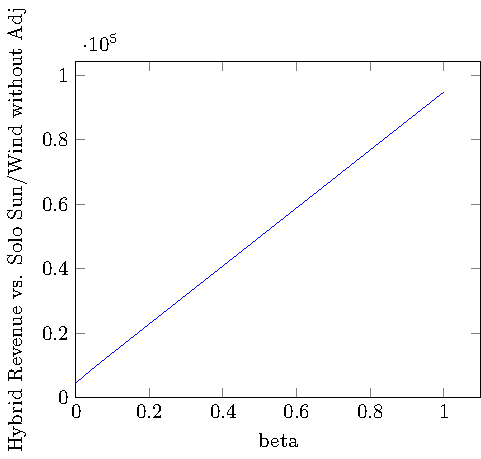
\includegraphics[]{Figures/figure2.pdf}}
		}
		\hfill
		\subfloat{
			\centering
			\scalebox{0.75}{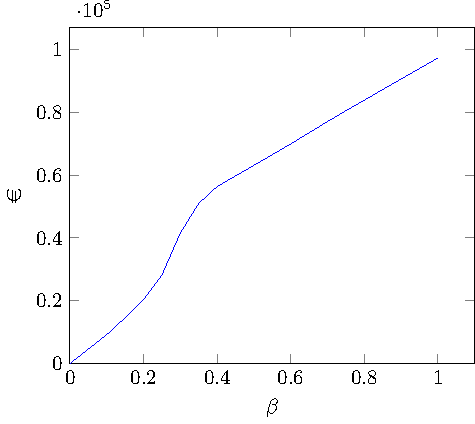
\includegraphics[]{Figures/figure.pdf}}
		}
		
		\caption{The difference of revenue between the hybrid energy producer and the sum of both individual producers' revenue depending on the risk-aversion factor $\beta$. On the left: The situation without an adjustment market. On the right: The situation with an adjustment market.  }\label{fig:overyear}
	\end{minipage}	
\end{figure}

We plotted the difference in the revenue of the hybrid producer and the sum of both single producers' revenues on the vertical axis. We presented the risk aversion factor $\beta$ on the horizontal axis. Overall, we see that the hybrid model is more advantageous for risk-averse producers. The more risk-averse a producer is, the more profitable it is to offer solar and wind power collectively. This is owed to having a larger mean while facing a lower variance in the collective production case. Hence, we can offer much more power for a given day-ahead price without facing more uncertainty. One striking difference is that the curve on the right starts in the origin whereas the curve on the left does not. If we have an adjustment market and are not risk-averse, it does not matter whether one producer offers both energies or two producers offer one energy each. The reason is that a risk-seeking producer offers everything on the day-ahead market and plans on buying back the deficit on the adjustment market. This is due to the producer expecting a lower price on the adjustment market $\mathbb{E}[\lambda_A]=30.45$ than on the day-ahead market $\mathbb{E}[\lambda_D]=32$ for our given data set.
On the other hand, if we do not have an adjustment market, we can exploit the anti-correlation. Thus, the variance of the produced amount of energy decreases and therefore, the hybrid producer can offer more energy for a given day-ahead price. Hence, it is more profitable to produce both collectively. 

Apart from that, we observe a linear growth behaviour in a market system without an adjustment market. When adding the adjustment market to the system, we notice a slight bump. At some value for the risk aversion factor $\beta$, the producer is not brave enough anymore to trade on arbitrage since he would face losses in specific scenarios. 



 
 %Section 4 Conclusion
 \section{Conclusion}

As an overall result, we see that a hybrid energy production model is more profitable than offering both energy resources separately. We also see that the hybrid producer's advantage increases the more risk-averse the producer is. This may be caused by the fact that a producer can offer more power for a given day-ahead price than a single energy producer. This follows since the mean of the hybrid producer's energy production sums up while the variance does not. However, the variance is smaller than the sum of both separately. The anti-correlation of both energy resources causes this effect. 
Even if the case study only focuses on a single period and not a time period over a whole year, it may also be a positive effect that the whole year power production faces smaller variance due to the even stronger anti-correlation of solar irradiance and wind power over the year. 

While the case study is based on a time series analysis on historical data for sun and wind energy production, the prices and ratios for day-ahead, adjustment, and balancing prices are taken from the example presented in Chapter 6 of \cite{Conejo10} . It may be worth to fully analyse a more realistic scenario setting and conduct case study over an entire year as we only focused on time period of one day. Another drawback of this survey is that the model faces some simplifications and assumptions. It may be interesting to extend the model to achieve a more realistic environment.  
 

 \bibliographystyle{plain}
 \bibliography{libary}


\end{document}

